\begin{figure*}[t!]
%\vspace{-20px}
\centering
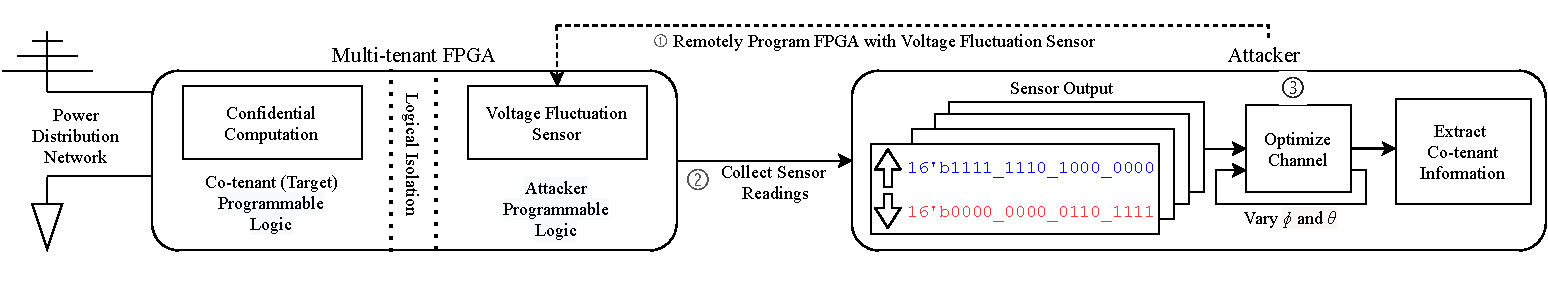
\includegraphics[width=\linewidth]{img/remote-tdc-attack.pdf}
\vspace{-30px}
\caption{Remote TDC Threat Model: \raisebox{.5pt}{\textcircled{\raisebox{-.8pt} {1}}} An attacker is given access to a remote multi-tenant FPGA and programs it with a \sensor. \raisebox{.5pt}{\textcircled{\raisebox{-.8pt} {2}}} The sensor readings are gathered and sent to the attacker for analysis. \raisebox{.5pt}{\textcircled{\raisebox{-.8pt} {3}}} The attacker tunes the parameters $\theta$ and $\phi$ to better extract co-tenant information. This paper studies the impact of $\theta$ and $\phi$ tuning.}

\vspace{-5px}
\label{fig:remote-tdc-attack}
\end{figure*}